




Besides and because of the exponential growth of data, the future data centers will have to change how they provide services to their users.
Many of the more important data sets are distributed through the Earth System Grid Federation (ESGF).
But at the moment analyzing the data is in many situations cumbersome and associated with a lot of overhead.
For example to apply CDOs it is necessary to download large data sets.
In many cases such a  download includes information the particular analysis is not concerned with.
\cite{tsengdar_lee_challenging_2013} lays out many of the concerns at NASA which would like to consolidate the data formats and also improve the tools used to constrain the models.
% obs4mips
Part of this vision is to provide platforms for science as a service as is tried in the NASA Earth Exchange (NEX).




%	\item
%	distributed approaches.. data is far away from where is generated, where users are using it
%	thus data locality
%	=> caches


Accelerated Climate Modeling for Energy (ACME) Ten Year Plan outlines a rough roadmap\cite{bader_accelerated_2014} on when to expect the rollout for different system size milestones. So while this is a US roadmap it seems reasonable to see similar trends in Europe.
The ACME strategy expected to utilize the first petascale systems by 2016 and expects the first exascale system by 2021.
A main factor for the considerations of this road map are of course the power budget constrains as implied by the 20MW limit.
The report also anticipates higher degrees of parallelism through the increased used of manycore architectures and the impact big data for analysis of climate data might have on the system design.


\begin{figure}[]
	\centering
	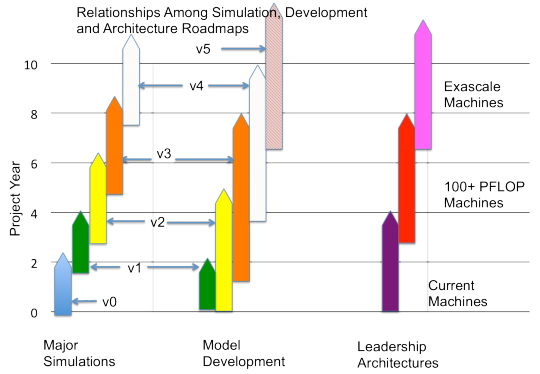
\includegraphics[width=0.66\textwidth]{3rd/acme2014_page7}
	\caption{ACME Roadmap for simulations, models and architectures. \cite{bader_accelerated_2014}}
	\label{fig:acme roadmap}
\end{figure}



Model resolution increases lead to substantial increases in data produced, but at least such resolution increases are not generally


These influences can be seen in a direct comparison of the 



To allow for authoritative forecasts not a single but a variety of different models are employed which are then combined into so called ensembles by the Climate Model Intercomparison Project (CMIP). 

\begin{itemize}
	\item \emph{CMIP3} as part of the Fourth IPCC Assessment Report (AR4) \cite{ipcc_ipcc_2010}. \\
	Models resolutions as computed at DKRZ:

	\begin{itemize}
		\item Atmosphere: 200km, 31 vertical layers
		\item Ocean between 10 and 150km
	\end{itemize}

	\item \emph{CMIP5} as part of the Fifth IPCC Assessment Report (AR5) \cite{ipcc_ipcc_2013}. \\
		Models resolutions as computed at DKRZ:

	\begin{itemize}
		\item Atmosphere: 200km, 47 layers
		\item Land: 200km, 47 layers
		\item Ocean: 12-150km, 40 layers
	\end{itemize}


\end{itemize}




%active satellites contributing to data used for climate modeling?
%	NASA +  ESA ... + ?


%
%
%four major challenges on the roadmap to exascale
%cite DARPA
%
%
%Energy and Power
%Memory and Storage
%Conurrency and Locality
%and Resilience.

